% Options for packages loaded elsewhere
\PassOptionsToPackage{unicode}{hyperref}
\PassOptionsToPackage{hyphens}{url}
%
\documentclass[
]{article}
\usepackage{amsmath,amssymb}
\usepackage{lmodern}
\usepackage{iftex}
\ifPDFTeX
  \usepackage[T1]{fontenc}
  \usepackage[utf8]{inputenc}
  \usepackage{textcomp} % provide euro and other symbols
\else % if luatex or xetex
  \usepackage{unicode-math}
  \defaultfontfeatures{Scale=MatchLowercase}
  \defaultfontfeatures[\rmfamily]{Ligatures=TeX,Scale=1}
\fi
% Use upquote if available, for straight quotes in verbatim environments
\IfFileExists{upquote.sty}{\usepackage{upquote}}{}
\IfFileExists{microtype.sty}{% use microtype if available
  \usepackage[]{microtype}
  \UseMicrotypeSet[protrusion]{basicmath} % disable protrusion for tt fonts
}{}
\makeatletter
\@ifundefined{KOMAClassName}{% if non-KOMA class
  \IfFileExists{parskip.sty}{%
    \usepackage{parskip}
  }{% else
    \setlength{\parindent}{0pt}
    \setlength{\parskip}{6pt plus 2pt minus 1pt}}
}{% if KOMA class
  \KOMAoptions{parskip=half}}
\makeatother
\usepackage{xcolor}
\IfFileExists{xurl.sty}{\usepackage{xurl}}{} % add URL line breaks if available
\IfFileExists{bookmark.sty}{\usepackage{bookmark}}{\usepackage{hyperref}}
\hypersetup{
  pdftitle={PSTAT131HW05},
  pdfauthor={Yifei Zhang},
  hidelinks,
  pdfcreator={LaTeX via pandoc}}
\urlstyle{same} % disable monospaced font for URLs
\usepackage[margin=1in]{geometry}
\usepackage{color}
\usepackage{fancyvrb}
\newcommand{\VerbBar}{|}
\newcommand{\VERB}{\Verb[commandchars=\\\{\}]}
\DefineVerbatimEnvironment{Highlighting}{Verbatim}{commandchars=\\\{\}}
% Add ',fontsize=\small' for more characters per line
\usepackage{framed}
\definecolor{shadecolor}{RGB}{248,248,248}
\newenvironment{Shaded}{\begin{snugshade}}{\end{snugshade}}
\newcommand{\AlertTok}[1]{\textcolor[rgb]{0.94,0.16,0.16}{#1}}
\newcommand{\AnnotationTok}[1]{\textcolor[rgb]{0.56,0.35,0.01}{\textbf{\textit{#1}}}}
\newcommand{\AttributeTok}[1]{\textcolor[rgb]{0.77,0.63,0.00}{#1}}
\newcommand{\BaseNTok}[1]{\textcolor[rgb]{0.00,0.00,0.81}{#1}}
\newcommand{\BuiltInTok}[1]{#1}
\newcommand{\CharTok}[1]{\textcolor[rgb]{0.31,0.60,0.02}{#1}}
\newcommand{\CommentTok}[1]{\textcolor[rgb]{0.56,0.35,0.01}{\textit{#1}}}
\newcommand{\CommentVarTok}[1]{\textcolor[rgb]{0.56,0.35,0.01}{\textbf{\textit{#1}}}}
\newcommand{\ConstantTok}[1]{\textcolor[rgb]{0.00,0.00,0.00}{#1}}
\newcommand{\ControlFlowTok}[1]{\textcolor[rgb]{0.13,0.29,0.53}{\textbf{#1}}}
\newcommand{\DataTypeTok}[1]{\textcolor[rgb]{0.13,0.29,0.53}{#1}}
\newcommand{\DecValTok}[1]{\textcolor[rgb]{0.00,0.00,0.81}{#1}}
\newcommand{\DocumentationTok}[1]{\textcolor[rgb]{0.56,0.35,0.01}{\textbf{\textit{#1}}}}
\newcommand{\ErrorTok}[1]{\textcolor[rgb]{0.64,0.00,0.00}{\textbf{#1}}}
\newcommand{\ExtensionTok}[1]{#1}
\newcommand{\FloatTok}[1]{\textcolor[rgb]{0.00,0.00,0.81}{#1}}
\newcommand{\FunctionTok}[1]{\textcolor[rgb]{0.00,0.00,0.00}{#1}}
\newcommand{\ImportTok}[1]{#1}
\newcommand{\InformationTok}[1]{\textcolor[rgb]{0.56,0.35,0.01}{\textbf{\textit{#1}}}}
\newcommand{\KeywordTok}[1]{\textcolor[rgb]{0.13,0.29,0.53}{\textbf{#1}}}
\newcommand{\NormalTok}[1]{#1}
\newcommand{\OperatorTok}[1]{\textcolor[rgb]{0.81,0.36,0.00}{\textbf{#1}}}
\newcommand{\OtherTok}[1]{\textcolor[rgb]{0.56,0.35,0.01}{#1}}
\newcommand{\PreprocessorTok}[1]{\textcolor[rgb]{0.56,0.35,0.01}{\textit{#1}}}
\newcommand{\RegionMarkerTok}[1]{#1}
\newcommand{\SpecialCharTok}[1]{\textcolor[rgb]{0.00,0.00,0.00}{#1}}
\newcommand{\SpecialStringTok}[1]{\textcolor[rgb]{0.31,0.60,0.02}{#1}}
\newcommand{\StringTok}[1]{\textcolor[rgb]{0.31,0.60,0.02}{#1}}
\newcommand{\VariableTok}[1]{\textcolor[rgb]{0.00,0.00,0.00}{#1}}
\newcommand{\VerbatimStringTok}[1]{\textcolor[rgb]{0.31,0.60,0.02}{#1}}
\newcommand{\WarningTok}[1]{\textcolor[rgb]{0.56,0.35,0.01}{\textbf{\textit{#1}}}}
\usepackage{graphicx}
\makeatletter
\def\maxwidth{\ifdim\Gin@nat@width>\linewidth\linewidth\else\Gin@nat@width\fi}
\def\maxheight{\ifdim\Gin@nat@height>\textheight\textheight\else\Gin@nat@height\fi}
\makeatother
% Scale images if necessary, so that they will not overflow the page
% margins by default, and it is still possible to overwrite the defaults
% using explicit options in \includegraphics[width, height, ...]{}
\setkeys{Gin}{width=\maxwidth,height=\maxheight,keepaspectratio}
% Set default figure placement to htbp
\makeatletter
\def\fps@figure{htbp}
\makeatother
\setlength{\emergencystretch}{3em} % prevent overfull lines
\providecommand{\tightlist}{%
  \setlength{\itemsep}{0pt}\setlength{\parskip}{0pt}}
\setcounter{secnumdepth}{-\maxdimen} % remove section numbering
\ifLuaTeX
  \usepackage{selnolig}  % disable illegal ligatures
\fi

\title{PSTAT131HW05}
\author{Yifei Zhang}
\date{2022-05-10}

\begin{document}
\maketitle

\begin{Shaded}
\begin{Highlighting}[]
\FunctionTok{library}\NormalTok{(ggplot2)}
\FunctionTok{library}\NormalTok{(tidyverse)}
\FunctionTok{library}\NormalTok{(tidymodels)}
\FunctionTok{library}\NormalTok{(corrplot)}
\FunctionTok{library}\NormalTok{(klaR)}
\FunctionTok{library}\NormalTok{(glmnet)}
\FunctionTok{tidymodels\_prefer}\NormalTok{()}
\NormalTok{Pokemon }\OtherTok{\textless{}{-}} \FunctionTok{read\_csv}\NormalTok{(}\StringTok{"Pokemon.csv"}\NormalTok{)}
\NormalTok{pokemon }\OtherTok{\textless{}{-}}\NormalTok{ readr}\SpecialCharTok{::}\FunctionTok{spec}\NormalTok{(Pokemon)}
\NormalTok{pokemon}
\end{Highlighting}
\end{Shaded}

\begin{verbatim}
## cols(
##   `#` = col_double(),
##   Name = col_character(),
##   `Type 1` = col_character(),
##   `Type 2` = col_character(),
##   Total = col_double(),
##   HP = col_double(),
##   Attack = col_double(),
##   Defense = col_double(),
##   `Sp. Atk` = col_double(),
##   `Sp. Def` = col_double(),
##   Speed = col_double(),
##   Generation = col_double(),
##   Legendary = col_logical()
## )
\end{verbatim}

\begin{Shaded}
\begin{Highlighting}[]
\FunctionTok{library}\NormalTok{(janitor)}
\end{Highlighting}
\end{Shaded}

\hypertarget{exercise-1}{%
\subsubsection{Exercise 1}\label{exercise-1}}

Install and load the \texttt{janitor} package. Use its
\texttt{clean\_names()} function on the Pokémon data, and save the
results to work with for the rest of the assignment. What happened to
the data? Why do you think \texttt{clean\_names()} is useful?

\begin{Shaded}
\begin{Highlighting}[]
\NormalTok{cleaned }\OtherTok{\textless{}{-}} \FunctionTok{clean\_names}\NormalTok{(Pokemon)}
\NormalTok{cleaned}
\end{Highlighting}
\end{Shaded}

\begin{verbatim}
## # A tibble: 800 x 13
##    number name      type_1 type_2 total    hp attack defense sp_atk sp_def speed
##     <dbl> <chr>     <chr>  <chr>  <dbl> <dbl>  <dbl>   <dbl>  <dbl>  <dbl> <dbl>
##  1      1 Bulbasaur Grass  Poison   318    45     49      49     65     65    45
##  2      2 Ivysaur   Grass  Poison   405    60     62      63     80     80    60
##  3      3 Venusaur  Grass  Poison   525    80     82      83    100    100    80
##  4      3 Venusaur~ Grass  Poison   625    80    100     123    122    120    80
##  5      4 Charmand~ Fire   <NA>     309    39     52      43     60     50    65
##  6      5 Charmele~ Fire   <NA>     405    58     64      58     80     65    80
##  7      6 Charizard Fire   Flying   534    78     84      78    109     85   100
##  8      6 Charizar~ Fire   Dragon   634    78    130     111    130     85   100
##  9      6 Charizar~ Fire   Flying   634    78    104      78    159    115   100
## 10      7 Squirtle  Water  <NA>     314    44     48      65     50     64    43
## # ... with 790 more rows, and 2 more variables: generation <dbl>,
## #   legendary <lgl>
\end{verbatim}

As the function name suggests, it cleaned the names of our Pokemon data,
made the names unique. I think clean\_names() is useful, because
sometime we may have variables with names that are very similar to each
other, and have space as a part of the name, which can cause a lot of
problems, and by using clean\_names() we can avoid these problems, and
we can change the letter case all at once.

\hypertarget{exercise-2}{%
\subsubsection{Exercise 2}\label{exercise-2}}

Using the entire data set, create a bar chart of the outcome variable,
\texttt{type\_1}.

\begin{Shaded}
\begin{Highlighting}[]
\NormalTok{count }\OtherTok{\textless{}{-}} \FunctionTok{table}\NormalTok{(cleaned}\SpecialCharTok{$}\NormalTok{type\_1)}
\NormalTok{count}
\end{Highlighting}
\end{Shaded}

\begin{verbatim}
## 
##      Bug     Dark   Dragon Electric    Fairy Fighting     Fire   Flying 
##       69       31       32       44       17       27       52        4 
##    Ghost    Grass   Ground      Ice   Normal   Poison  Psychic     Rock 
##       32       70       32       24       98       28       57       44 
##    Steel    Water 
##       27      112
\end{verbatim}

\begin{Shaded}
\begin{Highlighting}[]
\FunctionTok{barplot}\NormalTok{(count, }\AttributeTok{xlab =} \StringTok{"types"}\NormalTok{, }\AttributeTok{ylab =} \StringTok{"counts"}\NormalTok{, }\AttributeTok{main =}\StringTok{"type 1 counts"}\NormalTok{)}
\end{Highlighting}
\end{Shaded}

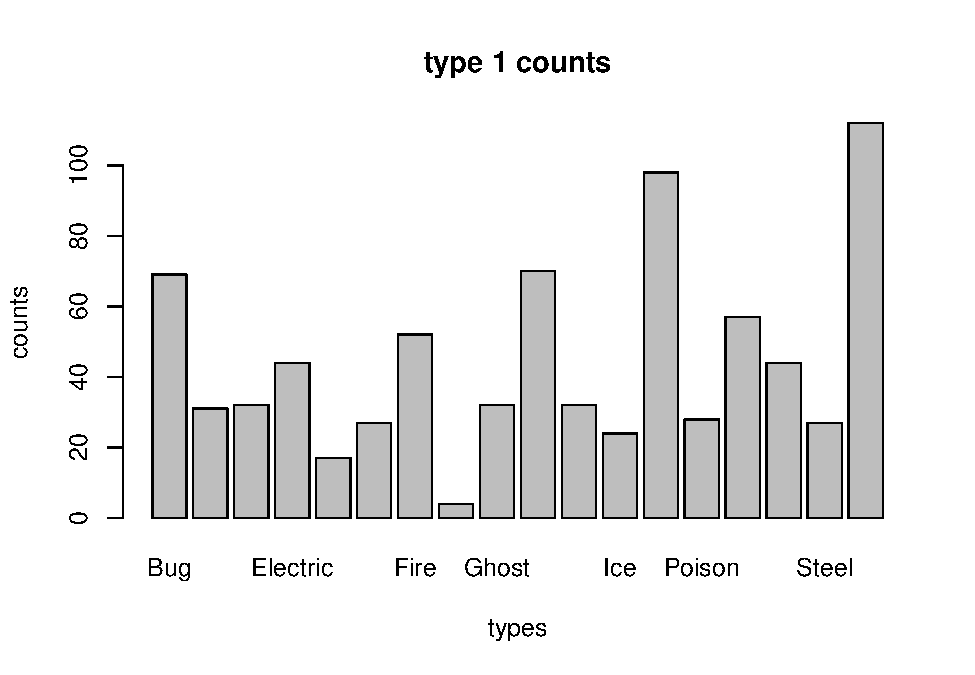
\includegraphics{PSTAT131HW05_files/figure-latex/unnamed-chunk-3-1.pdf}

\begin{Shaded}
\begin{Highlighting}[]
\CommentTok{\# not all the type names are shown in the xlab because thats too long}
\end{Highlighting}
\end{Shaded}

How many classes of the outcome are there? Are there any Pokémon types
with very few Pokémon? If so, which ones?

\begin{verbatim}
There are 18 class of outcomes. There are Pokémon types with very few Pokémon. Such as the  Flying class which only has 4,  Fairy with 17. There are a few other classes that are barely having above 20 pokemons. 
\end{verbatim}

For this assignment, we'll handle the rarer classes by simply filtering
them out. Filter the entire data set to contain only Pokémon whose
\texttt{type\_1} is Bug, Fire, Grass, Normal, Water, or Psychic.

\begin{Shaded}
\begin{Highlighting}[]
\NormalTok{filtered }\OtherTok{\textless{}{-}}\NormalTok{ cleaned }\SpecialCharTok{\%\textgreater{}\%} \FunctionTok{filter}\NormalTok{(}
\NormalTok{  type\_1 }\SpecialCharTok{==} \StringTok{"Bug"} \SpecialCharTok{|}\NormalTok{ type\_1 }\SpecialCharTok{==} \StringTok{"Fire"} \SpecialCharTok{|}\NormalTok{ type\_1 }\SpecialCharTok{==} \StringTok{"Grass"} 
  \SpecialCharTok{|}\NormalTok{ type\_1 }\SpecialCharTok{==} \StringTok{"Normal"} \SpecialCharTok{|}\NormalTok{ type\_1 }\SpecialCharTok{==} \StringTok{"Water"} \SpecialCharTok{|}\NormalTok{ type\_1 }\SpecialCharTok{==} \StringTok{"Psychic"}
\NormalTok{  )}
\NormalTok{filtered}
\end{Highlighting}
\end{Shaded}

\begin{verbatim}
## # A tibble: 458 x 13
##    number name      type_1 type_2 total    hp attack defense sp_atk sp_def speed
##     <dbl> <chr>     <chr>  <chr>  <dbl> <dbl>  <dbl>   <dbl>  <dbl>  <dbl> <dbl>
##  1      1 Bulbasaur Grass  Poison   318    45     49      49     65     65    45
##  2      2 Ivysaur   Grass  Poison   405    60     62      63     80     80    60
##  3      3 Venusaur  Grass  Poison   525    80     82      83    100    100    80
##  4      3 Venusaur~ Grass  Poison   625    80    100     123    122    120    80
##  5      4 Charmand~ Fire   <NA>     309    39     52      43     60     50    65
##  6      5 Charmele~ Fire   <NA>     405    58     64      58     80     65    80
##  7      6 Charizard Fire   Flying   534    78     84      78    109     85   100
##  8      6 Charizar~ Fire   Dragon   634    78    130     111    130     85   100
##  9      6 Charizar~ Fire   Flying   634    78    104      78    159    115   100
## 10      7 Squirtle  Water  <NA>     314    44     48      65     50     64    43
## # ... with 448 more rows, and 2 more variables: generation <dbl>,
## #   legendary <lgl>
\end{verbatim}

After filtering, convert \texttt{type\_1} and \texttt{legendary} to
factors.

\begin{Shaded}
\begin{Highlighting}[]
\NormalTok{data }\OtherTok{\textless{}{-}}\NormalTok{ filtered }\SpecialCharTok{\%\textgreater{}\%} 
  \FunctionTok{mutate}\NormalTok{(}\AttributeTok{type\_1 =} \FunctionTok{factor}\NormalTok{(type\_1),}
         \AttributeTok{legendary =} \FunctionTok{factor}\NormalTok{(legendary),}
         \AttributeTok{generation =} \FunctionTok{factor}\NormalTok{(generation)}
\NormalTok{         )}
\NormalTok{data}
\end{Highlighting}
\end{Shaded}

\begin{verbatim}
## # A tibble: 458 x 13
##    number name      type_1 type_2 total    hp attack defense sp_atk sp_def speed
##     <dbl> <chr>     <fct>  <chr>  <dbl> <dbl>  <dbl>   <dbl>  <dbl>  <dbl> <dbl>
##  1      1 Bulbasaur Grass  Poison   318    45     49      49     65     65    45
##  2      2 Ivysaur   Grass  Poison   405    60     62      63     80     80    60
##  3      3 Venusaur  Grass  Poison   525    80     82      83    100    100    80
##  4      3 Venusaur~ Grass  Poison   625    80    100     123    122    120    80
##  5      4 Charmand~ Fire   <NA>     309    39     52      43     60     50    65
##  6      5 Charmele~ Fire   <NA>     405    58     64      58     80     65    80
##  7      6 Charizard Fire   Flying   534    78     84      78    109     85   100
##  8      6 Charizar~ Fire   Dragon   634    78    130     111    130     85   100
##  9      6 Charizar~ Fire   Flying   634    78    104      78    159    115   100
## 10      7 Squirtle  Water  <NA>     314    44     48      65     50     64    43
## # ... with 448 more rows, and 2 more variables: generation <fct>,
## #   legendary <fct>
\end{verbatim}

\hypertarget{exercise-3}{%
\subsubsection{Exercise 3}\label{exercise-3}}

Perform an initial split of the data. Stratify by the outcome variable.
You can choose a proportion to use. Verify that your training and test
sets have the desired number of observations.

\begin{Shaded}
\begin{Highlighting}[]
\FunctionTok{set.seed}\NormalTok{(}\DecValTok{1010}\NormalTok{)}
\NormalTok{pokemon\_split }\OtherTok{\textless{}{-}}\NormalTok{ data }\SpecialCharTok{\%\textgreater{}\%} 
  \FunctionTok{initial\_split}\NormalTok{(}\AttributeTok{strata =}\NormalTok{ type\_1, }\AttributeTok{prop =} \FloatTok{0.7}\NormalTok{)}
\NormalTok{pokemon\_train }\OtherTok{\textless{}{-}} \FunctionTok{training}\NormalTok{(pokemon\_split)}
\NormalTok{pokemon\_test }\OtherTok{\textless{}{-}} \FunctionTok{testing}\NormalTok{(pokemon\_split)}
\FunctionTok{dim}\NormalTok{(pokemon\_train)}
\end{Highlighting}
\end{Shaded}

\begin{verbatim}
## [1] 318  13
\end{verbatim}

\begin{verbatim}
There are 318 observations in our training set, which is roughly 70 percent of our filtered overall dataset.
\end{verbatim}

Next, use \emph{v}-fold cross-validation on the training set. Use 5
folds. Stratify the folds by \texttt{type\_1} as well. \emph{Hint: Look
for a \texttt{strata} argument.} Why might stratifying the folds be
useful?

\begin{Shaded}
\begin{Highlighting}[]
\NormalTok{pokemon\_folds }\OtherTok{\textless{}{-}} \FunctionTok{vfold\_cv}\NormalTok{(pokemon\_train, }\AttributeTok{v =} \DecValTok{5}\NormalTok{, }\AttributeTok{strata =} \StringTok{\textquotesingle{}type\_1\textquotesingle{}}\NormalTok{)}
\NormalTok{pokemon\_folds}
\end{Highlighting}
\end{Shaded}

\begin{verbatim}
## #  5-fold cross-validation using stratification 
## # A tibble: 5 x 2
##   splits           id   
##   <list>           <chr>
## 1 <split [252/66]> Fold1
## 2 <split [253/65]> Fold2
## 3 <split [253/65]> Fold3
## 4 <split [256/62]> Fold4
## 5 <split [258/60]> Fold5
\end{verbatim}

Stratifying the folds can be useful useful because we want to make sure
the cross validation reaches the result as realistic as possible.

\hypertarget{exercise-4}{%
\subsubsection{Exercise 4}\label{exercise-4}}

Set up a recipe to predict \texttt{type\_1} with \texttt{legendary},
\texttt{generation}, \texttt{sp\_atk}, \texttt{attack}, \texttt{speed},
\texttt{defense}, \texttt{hp}, and \texttt{sp\_def}.

\begin{itemize}
\item
  Dummy-code \texttt{legendary} and \texttt{generation};
\item
  Center and scale all predictors.
\end{itemize}

\begin{Shaded}
\begin{Highlighting}[]
\NormalTok{pokemon\_recipe }\OtherTok{\textless{}{-}} \FunctionTok{recipe}\NormalTok{(type\_1 }\SpecialCharTok{\textasciitilde{}}\NormalTok{ legendary }\SpecialCharTok{+}\NormalTok{ generation }\SpecialCharTok{+}\NormalTok{ sp\_atk }\SpecialCharTok{+}
\NormalTok{                           attack }\SpecialCharTok{+}\NormalTok{ speed }\SpecialCharTok{+}\NormalTok{ defense }\SpecialCharTok{+}\NormalTok{ hp }\SpecialCharTok{+}\NormalTok{ sp\_def,}
                         \AttributeTok{data =}\NormalTok{ pokemon\_train) }\SpecialCharTok{\%\textgreater{}\%}
  \FunctionTok{step\_dummy}\NormalTok{(}\FunctionTok{all\_nominal\_predictors}\NormalTok{()) }\SpecialCharTok{\%\textgreater{}\%} 
  \FunctionTok{step\_normalize}\NormalTok{(}\FunctionTok{all\_predictors}\NormalTok{()) }
\end{Highlighting}
\end{Shaded}

\hypertarget{exercise-5}{%
\subsubsection{Exercise 5}\label{exercise-5}}

We'll be fitting and tuning an elastic net, tuning \texttt{penalty} and
\texttt{mixture} (use \texttt{multinom\_reg} with the \texttt{glmnet}
engine).

Set up this model and workflow. Create a regular grid for
\texttt{penalty} and \texttt{mixture} with 10 levels each;
\texttt{mixture} should range from 0 to 1. For this assignment, we'll
let \texttt{penalty} range from -5 to 5 (it's log-scaled).

How many total models will you be fitting when you fit these models to
your folded data?

We will be fitting 500 models to our folded data.

\begin{Shaded}
\begin{Highlighting}[]
\NormalTok{elastic\_spec }\OtherTok{\textless{}{-}} 
  \FunctionTok{multinom\_reg}\NormalTok{(}\AttributeTok{penalty =} \FunctionTok{tune}\NormalTok{(), }\AttributeTok{mixture =} \FunctionTok{tune}\NormalTok{()) }\SpecialCharTok{\%\textgreater{}\%} 
  \FunctionTok{set\_mode}\NormalTok{(}\StringTok{"classification"}\NormalTok{) }\SpecialCharTok{\%\textgreater{}\%} 
  \FunctionTok{set\_engine}\NormalTok{(}\StringTok{"glmnet"}\NormalTok{)}

\NormalTok{elastic\_workflow }\OtherTok{\textless{}{-}} \FunctionTok{workflow}\NormalTok{() }\SpecialCharTok{\%\textgreater{}\%} 
  \FunctionTok{add\_recipe}\NormalTok{(pokemon\_recipe) }\SpecialCharTok{\%\textgreater{}\%} 
  \FunctionTok{add\_model}\NormalTok{(elastic\_spec)}

\NormalTok{penalty\_grid }\OtherTok{\textless{}{-}} \FunctionTok{grid\_regular}\NormalTok{(}\FunctionTok{penalty}\NormalTok{(}\AttributeTok{range =} \FunctionTok{c}\NormalTok{(}\SpecialCharTok{{-}}\DecValTok{5}\NormalTok{, }\DecValTok{5}\NormalTok{)), }
                             \FunctionTok{mixture}\NormalTok{(}\AttributeTok{range =} \FunctionTok{c}\NormalTok{(}\DecValTok{0}\NormalTok{, }\DecValTok{1}\NormalTok{)),}
                             \AttributeTok{levels =} \DecValTok{10}\NormalTok{)}
\NormalTok{penalty\_grid}
\end{Highlighting}
\end{Shaded}

\begin{verbatim}
## # A tibble: 100 x 2
##          penalty mixture
##            <dbl>   <dbl>
##  1      0.00001        0
##  2      0.000129       0
##  3      0.00167        0
##  4      0.0215         0
##  5      0.278          0
##  6      3.59           0
##  7     46.4            0
##  8    599.             0
##  9   7743.             0
## 10 100000              0
## # ... with 90 more rows
\end{verbatim}

\hypertarget{exercise-6}{%
\subsubsection{Exercise 6}\label{exercise-6}}

Fit the models to your folded data using \texttt{tune\_grid()}.

Use \texttt{autoplot()} on the results. What do you notice? Do larger or
smaller values of \texttt{penalty} and \texttt{mixture} produce better
accuracy and ROC AUC?

\begin{Shaded}
\begin{Highlighting}[]
\NormalTok{tune\_res }\OtherTok{\textless{}{-}} \FunctionTok{tune\_grid}\NormalTok{(}
\NormalTok{  elastic\_workflow,}
  \AttributeTok{resamples =}\NormalTok{ pokemon\_folds, }
  \AttributeTok{grid =}\NormalTok{ penalty\_grid}
\NormalTok{)}
\NormalTok{tune\_res}
\end{Highlighting}
\end{Shaded}

\begin{verbatim}
## # Tuning results
## # 5-fold cross-validation using stratification 
## # A tibble: 5 x 4
##   splits           id    .metrics           .notes          
##   <list>           <chr> <list>             <list>          
## 1 <split [252/66]> Fold1 <tibble [200 x 6]> <tibble [0 x 1]>
## 2 <split [253/65]> Fold2 <tibble [200 x 6]> <tibble [0 x 1]>
## 3 <split [253/65]> Fold3 <tibble [200 x 6]> <tibble [0 x 1]>
## 4 <split [256/62]> Fold4 <tibble [200 x 6]> <tibble [0 x 1]>
## 5 <split [258/60]> Fold5 <tibble [200 x 6]> <tibble [0 x 1]>
\end{verbatim}

\begin{Shaded}
\begin{Highlighting}[]
\FunctionTok{autoplot}\NormalTok{(tune\_res)}
\end{Highlighting}
\end{Shaded}

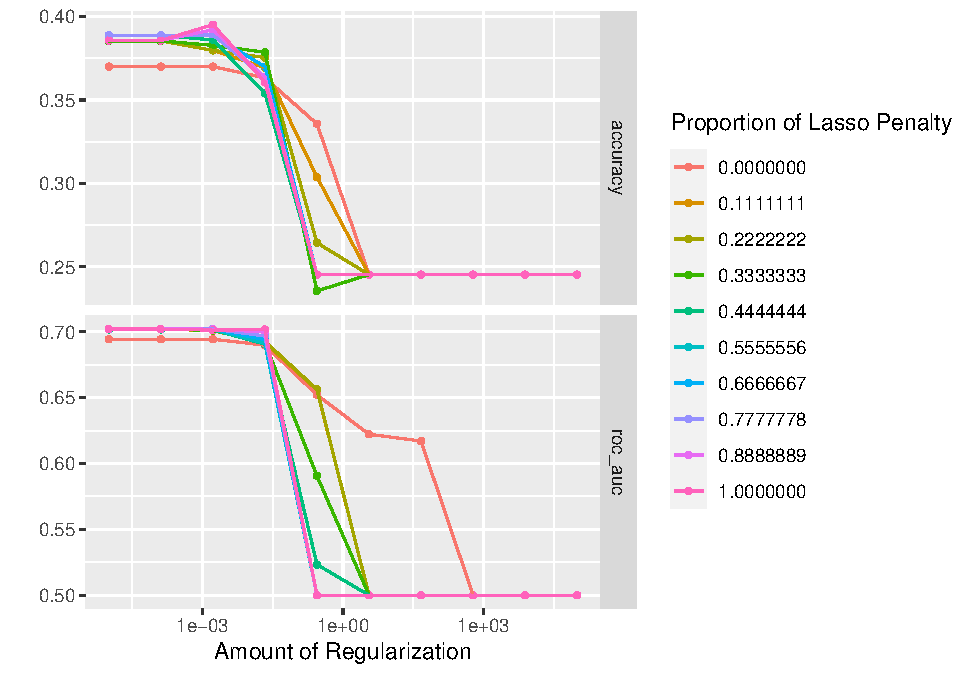
\includegraphics{PSTAT131HW05_files/figure-latex/unnamed-chunk-11-1.pdf}
lower penalty and higher mixture produce better accuracy and ROC AUC

\hypertarget{exercise-7}{%
\subsubsection{Exercise 7}\label{exercise-7}}

Use \texttt{select\_best()} to choose the model that has the optimal
\texttt{roc\_auc}. Then use \texttt{finalize\_workflow()},
\texttt{fit()}, and \texttt{augment()} to fit the model to the training
set and evaluate its performance on the testing set.

\begin{Shaded}
\begin{Highlighting}[]
\FunctionTok{collect\_metrics}\NormalTok{(tune\_res)}
\end{Highlighting}
\end{Shaded}

\begin{verbatim}
## # A tibble: 200 x 8
##     penalty mixture .metric  .estimator  mean     n std_err .config             
##       <dbl>   <dbl> <chr>    <chr>      <dbl> <int>   <dbl> <chr>               
##  1 0.00001        0 accuracy multiclass 0.370     5  0.0209 Preprocessor1_Model~
##  2 0.00001        0 roc_auc  hand_till  0.694     5  0.0141 Preprocessor1_Model~
##  3 0.000129       0 accuracy multiclass 0.370     5  0.0209 Preprocessor1_Model~
##  4 0.000129       0 roc_auc  hand_till  0.694     5  0.0141 Preprocessor1_Model~
##  5 0.00167        0 accuracy multiclass 0.370     5  0.0209 Preprocessor1_Model~
##  6 0.00167        0 roc_auc  hand_till  0.694     5  0.0141 Preprocessor1_Model~
##  7 0.0215         0 accuracy multiclass 0.363     5  0.0266 Preprocessor1_Model~
##  8 0.0215         0 roc_auc  hand_till  0.690     5  0.0147 Preprocessor1_Model~
##  9 0.278          0 accuracy multiclass 0.336     5  0.0173 Preprocessor1_Model~
## 10 0.278          0 roc_auc  hand_till  0.652     5  0.0126 Preprocessor1_Model~
## # ... with 190 more rows
\end{verbatim}

\begin{Shaded}
\begin{Highlighting}[]
\NormalTok{best\_penalty }\OtherTok{\textless{}{-}} \FunctionTok{select\_best}\NormalTok{(tune\_res, }\AttributeTok{metric =} \StringTok{"roc\_auc"}\NormalTok{)}
\NormalTok{best\_penalty}
\end{Highlighting}
\end{Shaded}

\begin{verbatim}
## # A tibble: 1 x 3
##   penalty mixture .config               
##     <dbl>   <dbl> <chr>                 
## 1 0.00001   0.889 Preprocessor1_Model081
\end{verbatim}

\begin{Shaded}
\begin{Highlighting}[]
\NormalTok{elastic\_final }\OtherTok{\textless{}{-}} \FunctionTok{finalize\_workflow}\NormalTok{(elastic\_workflow, best\_penalty)}

\NormalTok{elastic\_final\_fit }\OtherTok{\textless{}{-}} \FunctionTok{fit}\NormalTok{(elastic\_final, }\AttributeTok{data =}\NormalTok{ pokemon\_train)}

\FunctionTok{augment}\NormalTok{(elastic\_final\_fit, }\AttributeTok{new\_data =}\NormalTok{ pokemon\_test) }
\end{Highlighting}
\end{Shaded}

\begin{verbatim}
## # A tibble: 140 x 20
##    number name      type_1 type_2 total    hp attack defense sp_atk sp_def speed
##     <dbl> <chr>     <fct>  <chr>  <dbl> <dbl>  <dbl>   <dbl>  <dbl>  <dbl> <dbl>
##  1      1 Bulbasaur Grass  Poison   318    45     49      49     65     65    45
##  2      3 Venusaur  Grass  Poison   525    80     82      83    100    100    80
##  3      5 Charmele~ Fire   <NA>     405    58     64      58     80     65    80
##  4     10 Caterpie  Bug    <NA>     195    45     30      35     20     20    45
##  5     12 Butterfr~ Bug    Flying   395    60     45      50     90     80    70
##  6     15 Beedrill~ Bug    Poison   495    65    150      40     15     80   145
##  7     18 PidgeotM~ Normal Flying   579    83     80      80    135     80   121
##  8     39 Jigglypu~ Normal Fairy    270   115     45      20     45     25    20
##  9     44 Gloom     Grass  Poison   395    60     65      70     85     75    40
## 10     45 Vileplume Grass  Poison   490    75     80      85    110     90    50
## # ... with 130 more rows, and 9 more variables: generation <fct>,
## #   legendary <fct>, .pred_class <fct>, .pred_Bug <dbl>, .pred_Fire <dbl>,
## #   .pred_Grass <dbl>, .pred_Normal <dbl>, .pred_Psychic <dbl>,
## #   .pred_Water <dbl>
\end{verbatim}

\begin{Shaded}
\begin{Highlighting}[]
\FunctionTok{augment}\NormalTok{(elastic\_final\_fit, }\AttributeTok{new\_data =}\NormalTok{ pokemon\_test) }\SpecialCharTok{\%\textgreater{}\%}
  \FunctionTok{accuracy}\NormalTok{(}\AttributeTok{truth =}\NormalTok{ type\_1, }\AttributeTok{estimate =}\NormalTok{ .pred\_class}
\NormalTok{          )}
\end{Highlighting}
\end{Shaded}

\begin{verbatim}
## # A tibble: 1 x 3
##   .metric  .estimator .estimate
##   <chr>    <chr>          <dbl>
## 1 accuracy multiclass     0.393
\end{verbatim}

\hypertarget{exercise-8}{%
\subsubsection{Exercise 8}\label{exercise-8}}

Calculate the overall ROC AUC on the testing set.

Then create plots of the different ROC curves, one per level of the
outcome. Also make a heat map of the confusion matrix.

What do you notice? How did your model do? Which Pokemon types is the
model best at predicting, and which is it worst at? Do you have any
ideas why this might be?

\begin{Shaded}
\begin{Highlighting}[]
\FunctionTok{augment}\NormalTok{(elastic\_final\_fit, }\AttributeTok{new\_data =}\NormalTok{ pokemon\_test) }\SpecialCharTok{\%\textgreater{}\%}
  \FunctionTok{roc\_auc}\NormalTok{(}\AttributeTok{truth =}\NormalTok{ type\_1, }\AttributeTok{estimate =} \FunctionTok{c}\NormalTok{(.pred\_Bug, .pred\_Fire, }
\NormalTok{                                       .pred\_Grass, .pred\_Normal, }
\NormalTok{                                       .pred\_Psychic, .pred\_Water}
\NormalTok{                                       ))}
\end{Highlighting}
\end{Shaded}

\begin{verbatim}
## # A tibble: 1 x 3
##   .metric .estimator .estimate
##   <chr>   <chr>          <dbl>
## 1 roc_auc hand_till      0.702
\end{verbatim}

collect\_metrics(final\_fit) test\_acc \textless- augment(final\_fit,
new\_data = titanic\_train) \%\textgreater\% roc\_auc(truth = survived,
estimate = .pred\_class)

\begin{Shaded}
\begin{Highlighting}[]
\FunctionTok{augment}\NormalTok{(elastic\_final\_fit, }\AttributeTok{new\_data =}\NormalTok{ pokemon\_test) }\SpecialCharTok{\%\textgreater{}\%}
  \FunctionTok{roc\_curve}\NormalTok{(}\AttributeTok{truth =}\NormalTok{ type\_1, }\AttributeTok{estimate =} \FunctionTok{c}\NormalTok{(.pred\_Bug, .pred\_Fire, }
\NormalTok{                                       .pred\_Grass, .pred\_Normal, }
\NormalTok{                                       .pred\_Psychic, .pred\_Water}
\NormalTok{                                       ))}\SpecialCharTok{\%\textgreater{}\%}
              \FunctionTok{autoplot}\NormalTok{()}
\end{Highlighting}
\end{Shaded}

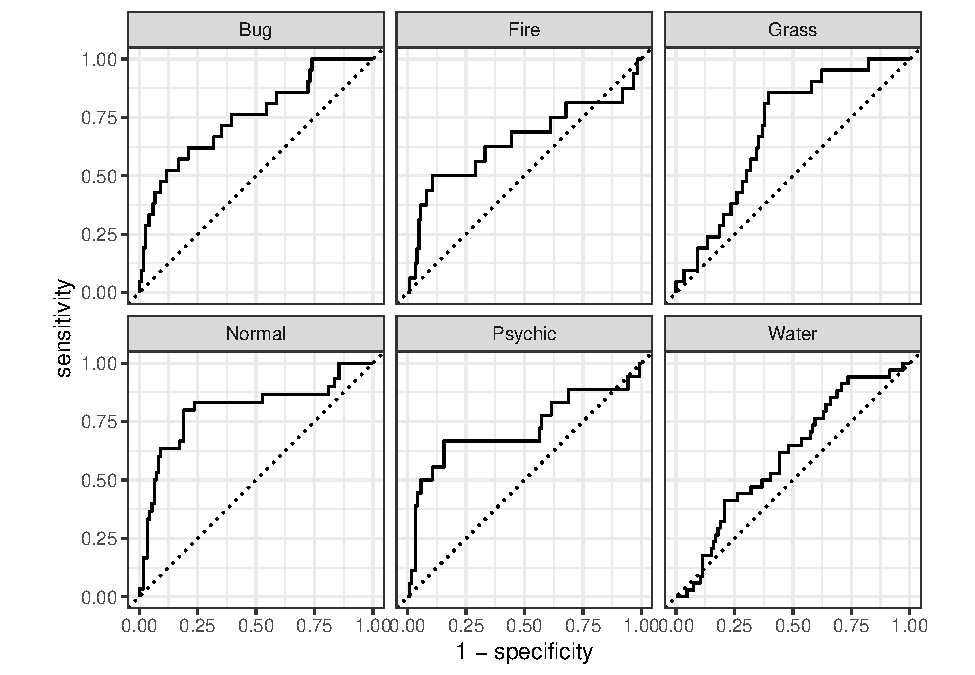
\includegraphics{PSTAT131HW05_files/figure-latex/unnamed-chunk-16-1.pdf}

\begin{Shaded}
\begin{Highlighting}[]
\FunctionTok{augment}\NormalTok{(elastic\_final\_fit, }\AttributeTok{new\_data =}\NormalTok{ pokemon\_test) }\SpecialCharTok{\%\textgreater{}\%}
  \FunctionTok{conf\_mat}\NormalTok{(}\AttributeTok{truth =}\NormalTok{ type\_1, }\AttributeTok{estimate =}\NormalTok{ .pred\_class) }\SpecialCharTok{\%\textgreater{}\%} 
  \FunctionTok{autoplot}\NormalTok{(}\AttributeTok{type =} \StringTok{"heatmap"}\NormalTok{)}
\end{Highlighting}
\end{Shaded}

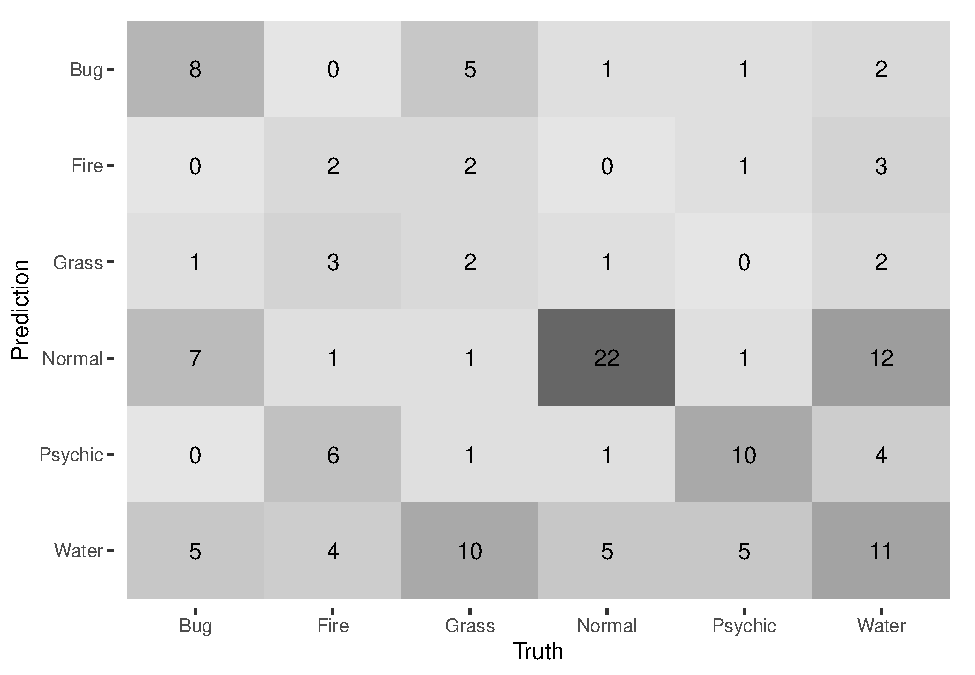
\includegraphics{PSTAT131HW05_files/figure-latex/unnamed-chunk-17-1.pdf}

It is hard to predict. The accuracy is lower than roc\_auc score.It did
better than I expected. Since the accuracy is low on the testing set for
the selected best model. Pokemon types that is the model best at
predicting is normal, Its worst at predicting water/ grass. They do not
have big enough number of them to begin with, so the estimations are way
off.

\end{document}
